% Created 2024-05-04 Sat 17:09
% Intended LaTeX compiler: lualatex
\documentclass[presentation]{beamer}
\usepackage{graphicx}
\usepackage{longtable}
\usepackage{wrapfig}
\usepackage{rotating}
\usepackage[normalem]{ulem}
\usepackage{amsmath}
\usepackage{amssymb}
\usepackage{capt-of}
\usepackage{hyperref}
\usetheme{default}
\author{fabio}
\date{\today}
\title{}
\hypersetup{
 pdfauthor={fabio},
 pdftitle={},
 pdfkeywords={},
 pdfsubject={},
 pdfcreator={Emacs 29.2 (Org mode 9.6.15)}, 
 pdflang={English}}
\begin{document}

\begin{frame}{Outline}
\tableofcontents
\end{frame}

\begin{frame}[label={sec:org524b6ef}]{Carboidratos}
\begin{block}{Carboidratos}
Os carboidratos são compostos orgânicos que contêm: \alert{C}, \alert{H} e \alert{O} em várias combinações

Conhecidos como açúcar ou sacarídeo, originária do Latim \emph{saccharum} e do Grego \emph{sakcharon}.

\begin{figure}[htbp]
\centering
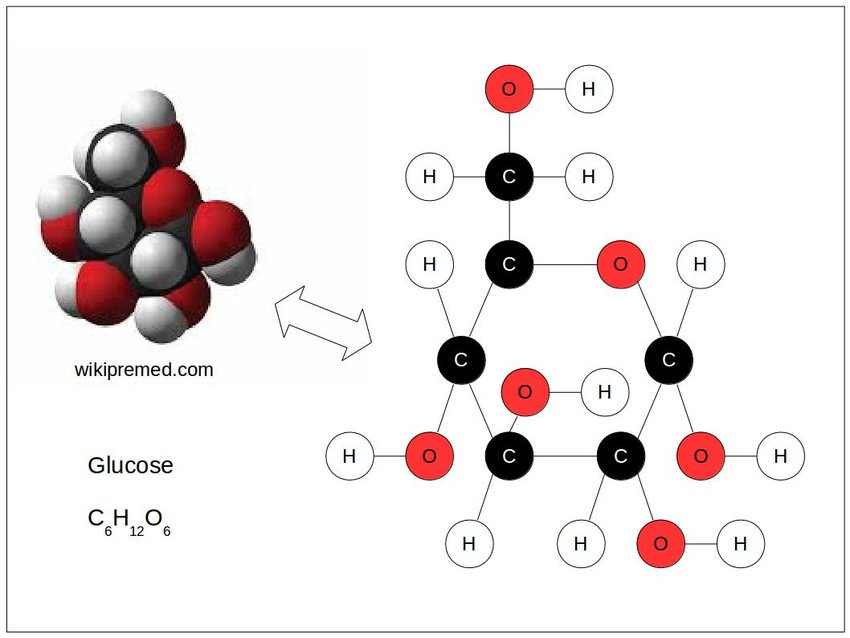
\includegraphics[scale=0.3]{./glucose.png}
\caption{Molécula da glicose composta por carbono, hidrogênio e oxigênio.}
\end{figure}
\end{block}





\begin{block}{Função}
\begin{columns}
\begin{column}{0.45\columnwidth}
\begin{block}{}
\begin{center}

\includegraphics[width=.9\linewidth]{./esteira.png}
\end{center}
\end{block}
\end{column}


\begin{column}{0.45\columnwidth}
\begin{block}{}
\begin{itemize}
\item Fornecimento de energia
\begin{bclogo}{Valores}
1g = 4 Kcal 
\end{bclogo}
\item Reserva de energia
\item Estrutural

\begin{center}
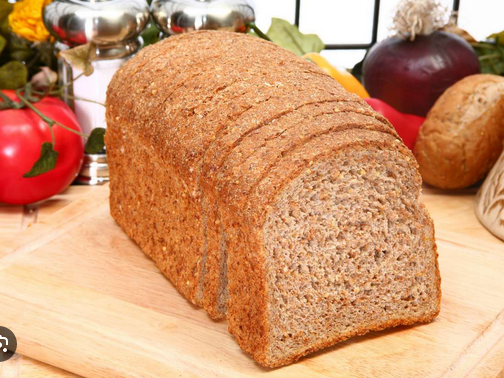
\includegraphics[scale=0.2]{./pao.png}
\end{center}
\end{itemize}
\end{block}
\end{column}
\end{columns}
\end{block}
\end{frame}
\end{document}
